%================================================================
\chapter{Results and Discussion}\label{chap:results_discussion}
%================================================================
In this chapter, we will detail how various models presented in previous chapters were configured and trained. The models will also be characterized using aforementioned numerical methods, and the results will be compared to earlier research.

The vanishing gradient phenomenon will be investigated for QCN and DNN models by studying the magnitude of their gradients (see \autoref{sec:BackwardPropagationQCN} and \autoref{sec:BackpropogationDNN}). This will be done for different architectures, especially different number of layers.

We will characterize the geometry of the loss landscape of QCNs(see \autoref{sec:Quantum Circuit Network}) and other models by studying the EFIM presented in \autoref{sec:EFIM}. The result will be used to asses the trainability of different models and predict how architecture affects training.

To assess the expressivity of QCNs and compare them to other models, we will use trajectory length as presented in \autoref{sec:TrajectoryLength}. This will be done for both trained and untrained models.

In order to test models in a practical setting, and give support to previous results and analyses in this thesis, the models will be trained to fit gaussian data. This will be done both using idealised simulation(see \autoref{sec:Exact Expectation Value}), and simulated, noisy hardware(see).


%================================================================
\section{Vanishing Gradient Phenomenon}\label{sec:Vanishing Gradient Phenomenon}
%================================================================


%================================================================
\section{Investigating the Loss Landscape}\label{sec:Investigating the Loss Landscape}
%================================================================
We explore the geometry of the loss landscape of various models by studying the eigenvalue spectrum of the EFIM \autoref{eq:EmpiricalFisher}. 


\begin{figure*}[t!]
    \centering
    \begin{subfigure}[t]{0.5\textwidth}
        \centering
        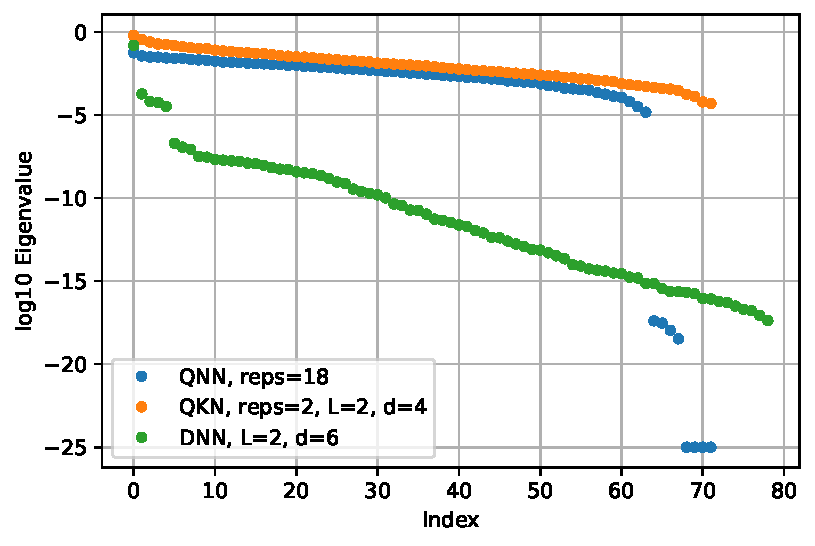
\includegraphics[height=1.4in]{latex/figures/FIM_qubits_4.pdf}
        \caption{Lorem ipsum}
    \end{subfigure}%
    ~ 
    \begin{subfigure}[t]{0.5\textwidth}
        \centering
        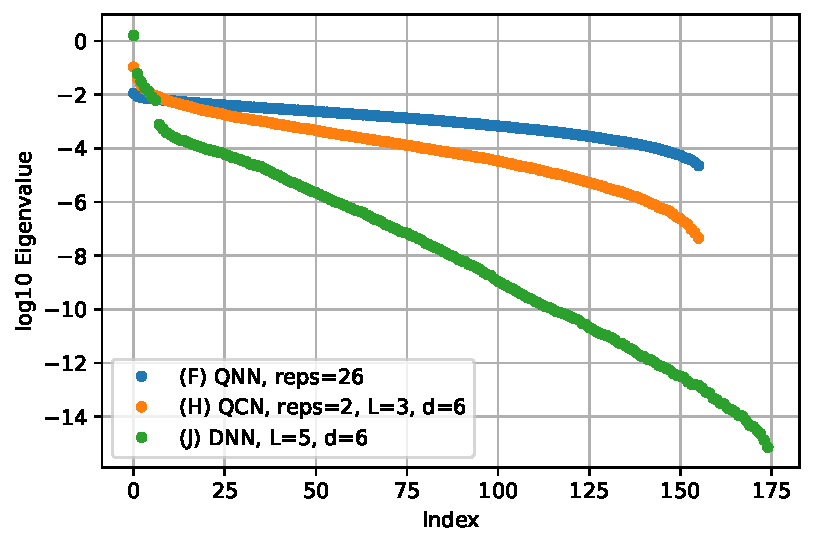
\includegraphics[width=1.4in]{latex/figures/FIM_qubits_6.pdf}
        \caption{Lorem ipsum}
    \end{subfigure}
    \caption{Caption place holder}
\end{figure*}

\begin{table}[]
\begin{tabular}{|l|l|l|l|l|l|}
\hline
Model &Type & Layers & Reps & Encoder        & $n_{\theta}$ \\ \hline
1a    & QNN & 1     & 18   & RZZ Encoding   & 72  \\ \hline
1b    & QCN & 2      & 3    & Qubit Encoding & 60 \\ \hline
1c    & QCN & 3      & 2    & Qubit Encoding & 72  \\ \hline
1d    & QCN & 5      & 1    & Qubit Encoding & 68  \\ \hline
1e    & DNN & 3      & NA   & NA             & 79 \\ \hline
\end{tabular}
\end{table}

%================================================================
\section{Expressivity of Untrained and Trained Models}\label{sec:Expressivity of Untrained and Trained Models}
%================================================================


%================================================================
\section{Training Models on Gaussian Data}\label{sec:Training Models on Gaussian Data}
%================================================================

